\documentclass{standalone}
\usepackage[dvipsnames]{xcolor}
\usepackage{tikz}
\usepackage[export]{animate}
\usepackage{ifthen}
\definecolor{darkgreen}{RGB}{10,90,10}

\begin{document}
\begin{animateinline}[controls]{30}
%First push action
\multiframe{10}{i=0+9}{%
\begin{tikzpicture}[x=1cm, y=1cm]
	\path (-6.25,-6.25) to (6.25,6.25); 

	\node[draw, ultra thick, circle, minimum size=2cm, inner sep=0pt, fill=Blue] at (-1,1) {};
	\node[draw, ultra thick, circle, minimum size=2cm, inner sep=0pt, fill=Green] at (1,1) {};
	\node[draw, ultra thick, circle, minimum size=2cm, inner sep=0pt, fill=Purple] at (-1,-1) {};
	\node[draw, ultra thick, circle, minimum size=2cm, inner sep=0pt, fill=Red] at (1,-1) {};
	\node[draw, ultra thick, circle, minimum size=2cm, inner sep=0pt, fill=Yellow, rotate around={\i:(0,-4)}] at (1,5) {};

\end{tikzpicture}}
\newframe
\multiframe{10}{r=0+0.2}{%
\begin{tikzpicture}[x=1cm, y=1cm]
	\path (-6.25,-6.25) to (6.25,6.25); 

	\node[draw, ultra thick, circle, minimum size=2cm, inner sep=0pt, fill=Blue] at (-1+\r,1) {};
	\node[draw, ultra thick, circle, minimum size=2cm, inner sep=0pt, fill=Green] at (1+\r,1) {};
	\node[draw, ultra thick, circle, minimum size=2cm, inner sep=0pt, fill=Purple] at (-1,-1) {};
	\node[draw, ultra thick, circle, minimum size=2cm, inner sep=0pt, fill=Red] at (1,-1) {};
	\node[draw, ultra thick, circle, minimum size=2cm, inner sep=0pt, fill=Yellow] at (-3+\r,1) {};

\end{tikzpicture}}
\newframe
\multiframe{10}{r=0+0.1}{%
\begin{tikzpicture}[x=1cm, y=1cm]
	\path (-6.25,-6.25) to (6.25,6.25); 

	\node[draw, ultra thick, circle, minimum size=2cm, inner sep=0pt, fill=Blue] at (1,1) {};
	\node[draw, ultra thick, circle, minimum size=2cm, inner sep=0pt, fill=Green] at (3+2*\r,1-2*\r) {};
	\node[draw, ultra thick, circle, minimum size=2cm, inner sep=0pt, fill=Purple] at (-1,-1) {};
	\node[draw, ultra thick, circle, minimum size=2cm, inner sep=0pt, fill=Red] at (1,-1) {};
	\node[draw, ultra thick, circle, minimum size=2cm, inner sep=0pt, fill=Yellow] at (-1,1) {};

\end{tikzpicture}}

\newframe
\multiframe{30}{i=0+9}{%
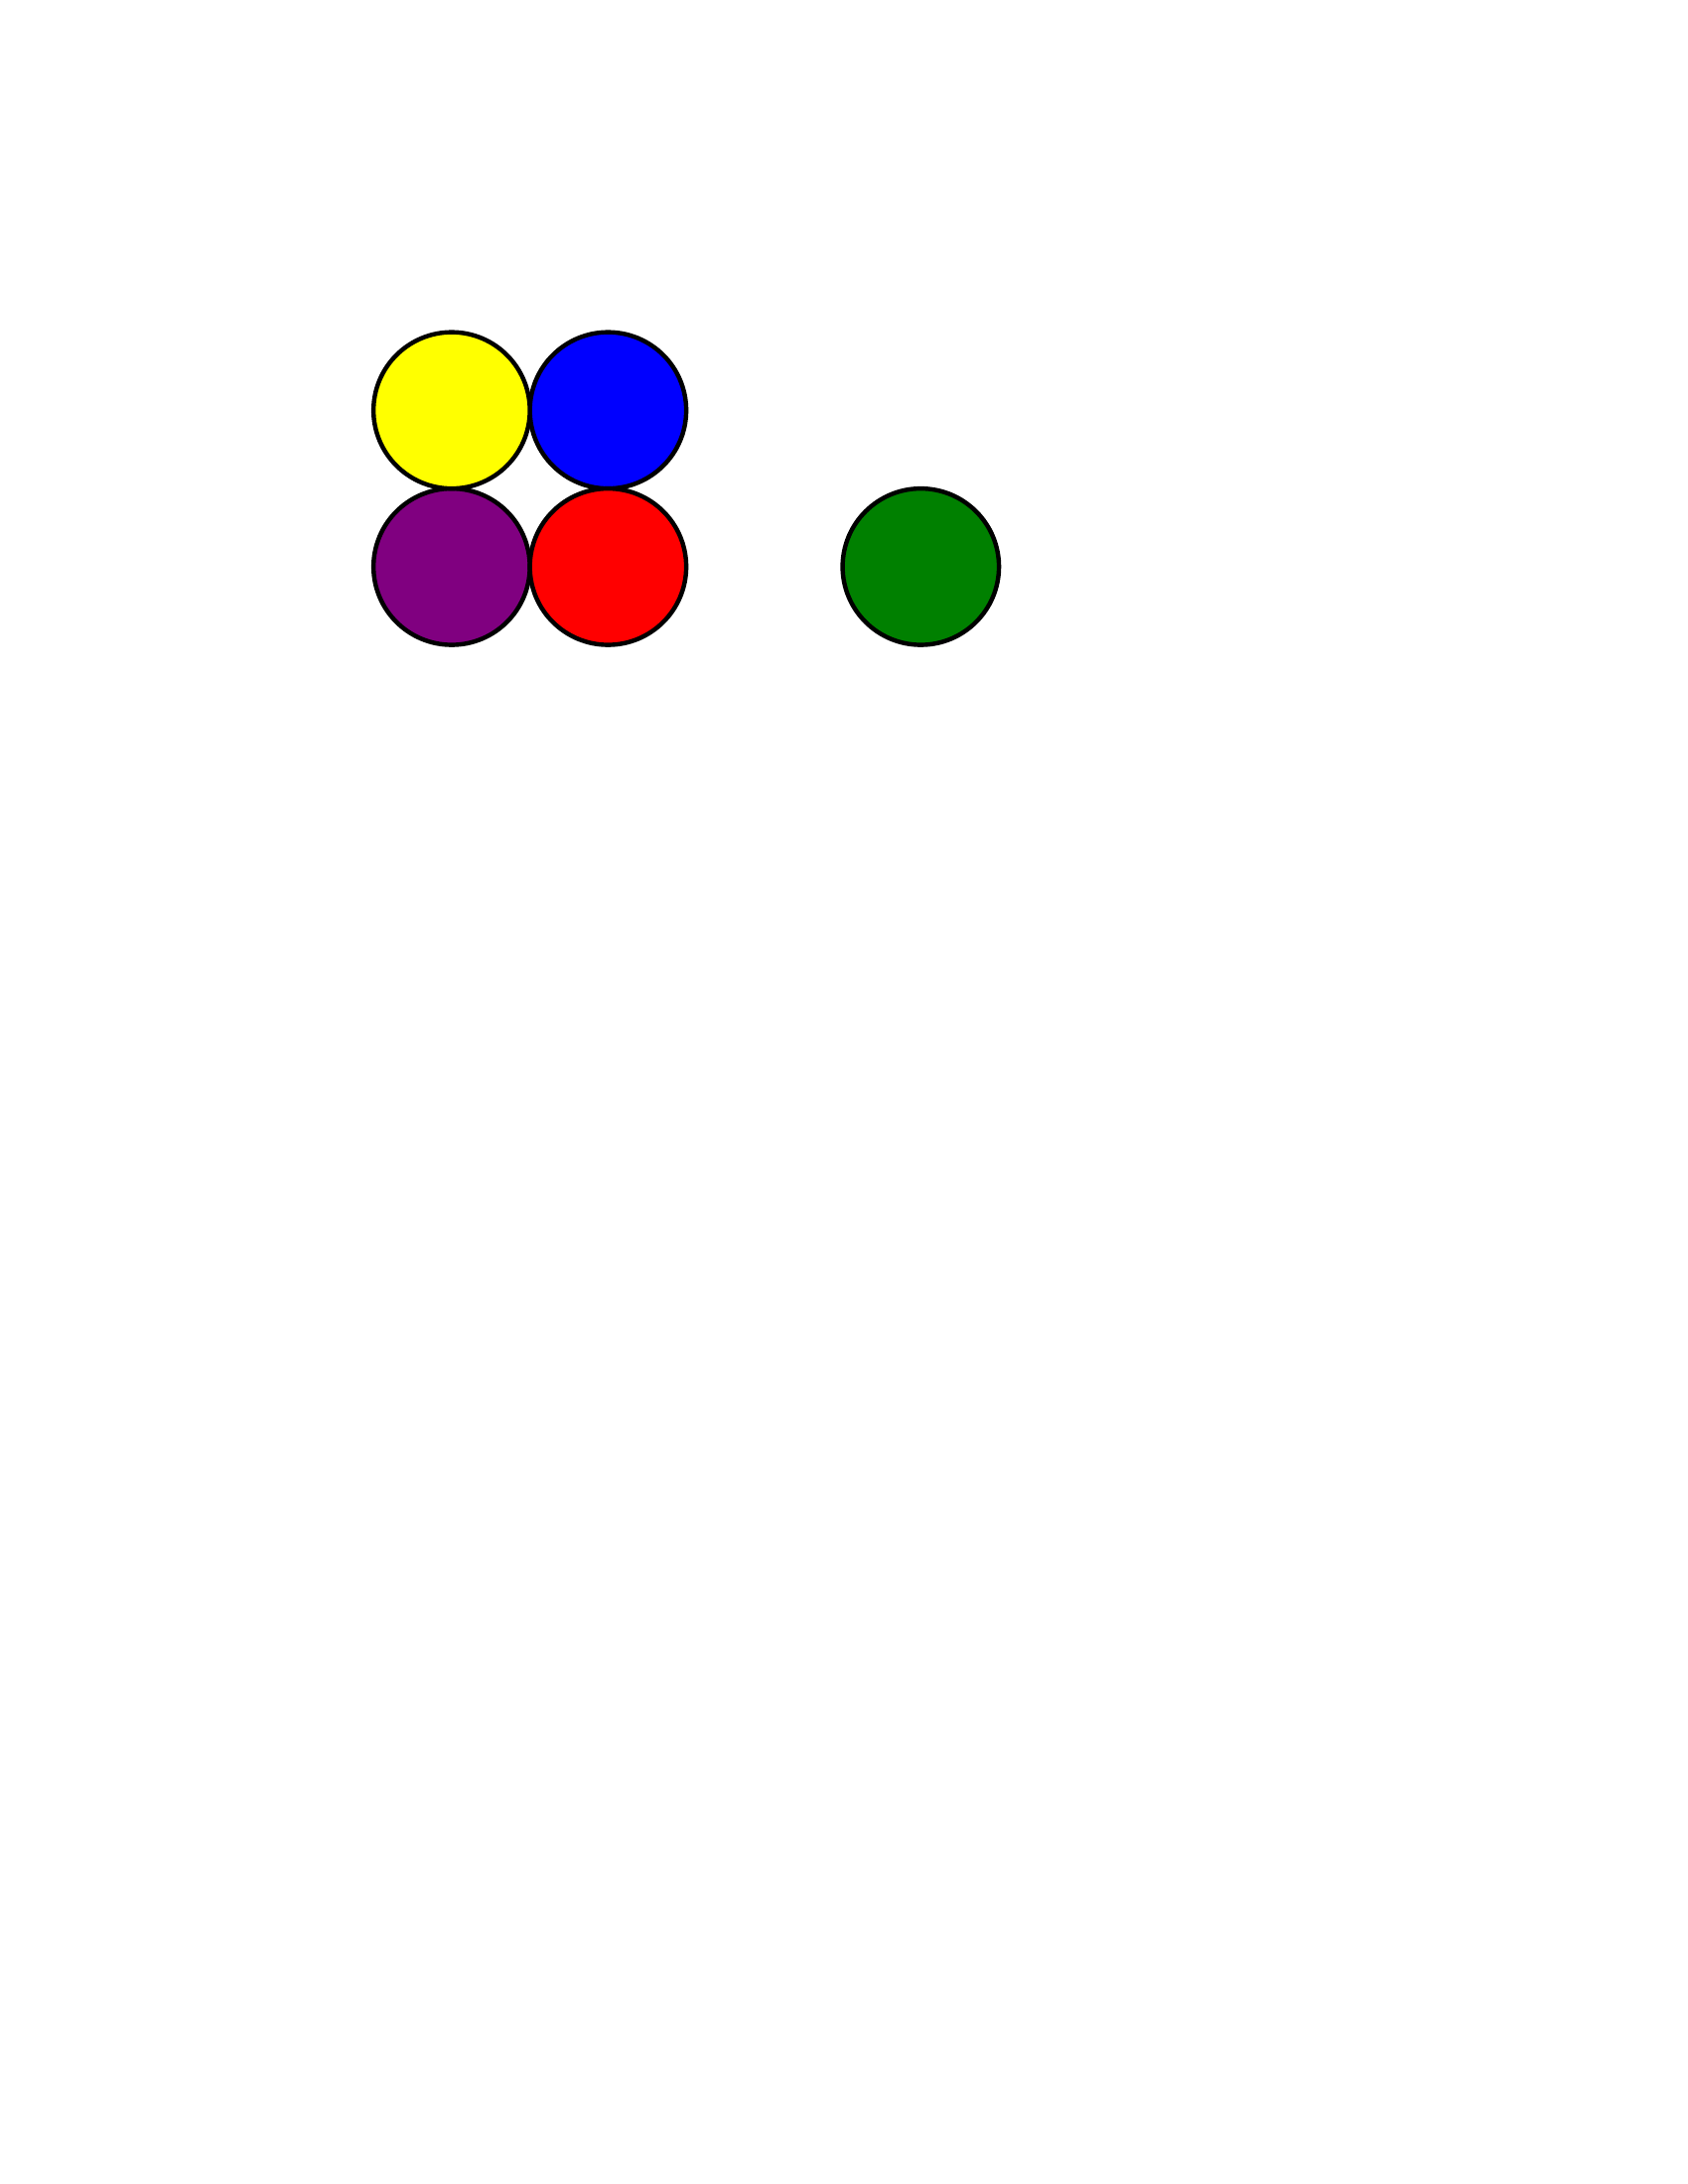
\begin{tikzpicture}[x=1cm, y=1cm]
	\path (-6.25,-6.25) to (6.25,6.25); 

	\node[draw, ultra thick, circle, minimum size=2cm, inner sep=0pt, fill=Blue] at (1,1) {};
	\node[draw, ultra thick, circle, minimum size=2cm, inner sep=0pt, fill=Green] at (5,-1) {};
	\node[draw, ultra thick, circle, minimum size=2cm, inner sep=0pt, fill=Purple] at (-1,-1) {};
	\node[draw, ultra thick, circle, minimum size=2cm, inner sep=0pt, fill=Red] at (1,-1) {};
	\node[draw, ultra thick, circle, minimum size=2cm, inner sep=0pt, fill=Yellow] at (-1,1) {};
\end{tikzpicture}}

% Second Push action

\newframe
\multiframe{10}{i=0+9}{%
\begin{tikzpicture}[x=1cm, y=1cm]
	\path (-6.25,-6.25) to (6.25,6.25); 

	\node[draw, ultra thick, circle, minimum size=2cm, inner sep=0pt, fill=Blue] at (1,1) {};
	\node[draw, ultra thick, circle, minimum size=2cm, inner sep=0pt, fill=Green, rotate around={\i:(-4,0)}] at (5,-1) {};
	\node[draw, ultra thick, circle, minimum size=2cm, inner sep=0pt, fill=Purple] at (-1,-1) {};
	\node[draw, ultra thick, circle, minimum size=2cm, inner sep=0pt, fill=Red] at (1,-1) {};
	\node[draw, ultra thick, circle, minimum size=2cm, inner sep=0pt, fill=Yellow] at (-1,1) {};

\end{tikzpicture}}
\newframe
\multiframe{10}{r=0+0.2}{%
\begin{tikzpicture}[x=1cm, y=1cm]
	\path (-6.25,-6.25) to (6.25,6.25); 

	\node[draw, ultra thick, circle, minimum size=2cm, inner sep=0pt, fill=Blue] at (1,1-\r) {};
	\node[draw, ultra thick, circle, minimum size=2cm, inner sep=0pt, fill=Green] at (1,3-\r) {};
	\node[draw, ultra thick, circle, minimum size=2cm, inner sep=0pt, fill=Purple] at (-1,-1) {};
	\node[draw, ultra thick, circle, minimum size=2cm, inner sep=0pt, fill=Red] at (1,-1-\r) {};
	\node[draw, ultra thick, circle, minimum size=2cm, inner sep=0pt, fill=Yellow] at (-1,1) {};

\end{tikzpicture}}
\newframe
\multiframe{10}{r=0+0.1}{%
\begin{tikzpicture}[x=1cm, y=1cm]
	\path (-6.25,-6.25) to (6.25,6.25); 

	\node[draw, ultra thick, circle, minimum size=2cm, inner sep=0pt, fill=Blue] at (1,-1) {};
	\node[draw, ultra thick, circle, minimum size=2cm, inner sep=0pt, fill=Green] at (1,1) {};
	\node[draw, ultra thick, circle, minimum size=2cm, inner sep=0pt, fill=Purple] at (-1,-1) {};
	\node[draw, ultra thick, circle, minimum size=2cm, inner sep=0pt, fill=Red] at (1-2*\r,-3-2*\r) {};
	\node[draw, ultra thick, circle, minimum size=2cm, inner sep=0pt, fill=Yellow] at (-1,1) {};

\end{tikzpicture}}
\newframe
\multiframe{30}{i=0+9}{%
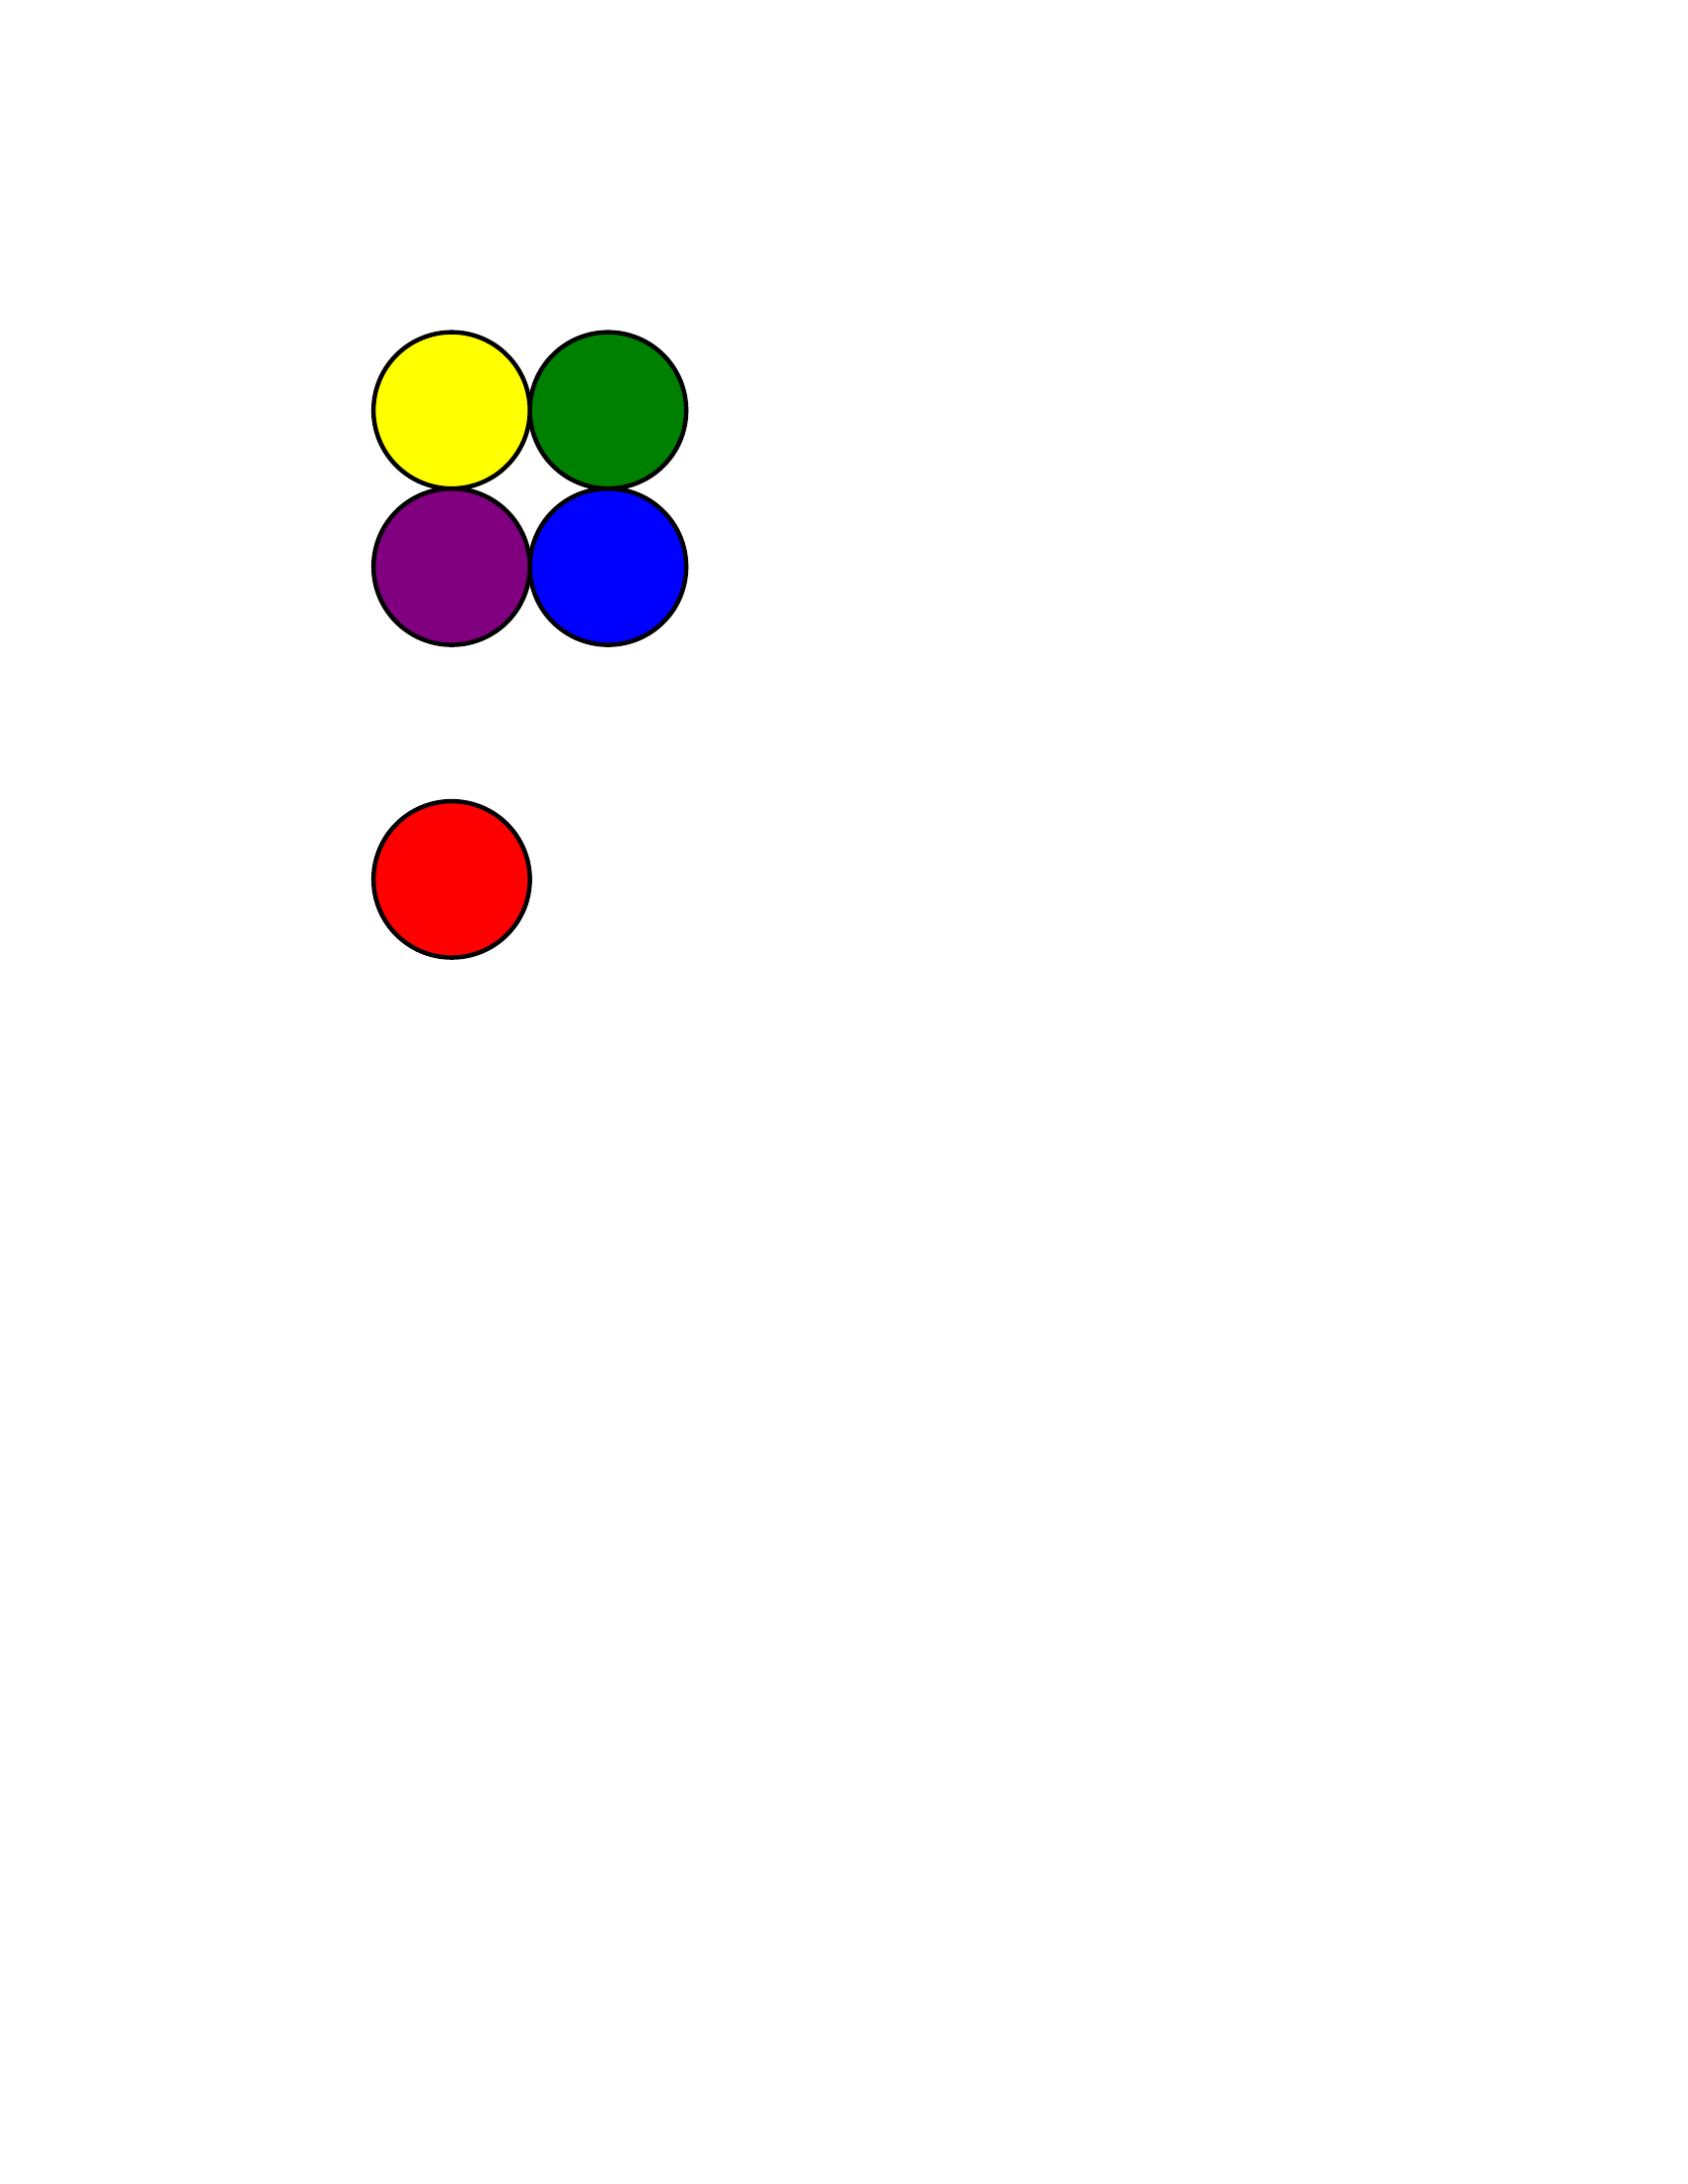
\begin{tikzpicture}[x=1cm, y=1cm]
	\path (-6.25,-6.25) to (6.25,6.25); 

	\node[draw, ultra thick, circle, minimum size=2cm, inner sep=0pt, fill=Blue] at (1,-1) {};
	\node[draw, ultra thick, circle, minimum size=2cm, inner sep=0pt, fill=Green] at (1,1) {};
	\node[draw, ultra thick, circle, minimum size=2cm, inner sep=0pt, fill=Purple] at (-1,-1) {};
	\node[draw, ultra thick, circle, minimum size=2cm, inner sep=0pt, fill=Red] at (-1,-5) {};
	\node[draw, ultra thick, circle, minimum size=2cm, inner sep=0pt, fill=Yellow] at (-1,1) {};

\end{tikzpicture}}

% Third push action

\newframe
\multiframe{10}{i=0+9}{%
\begin{tikzpicture}[x=1cm, y=1cm]
	\path (-6.25,-6.25) to (6.25,6.25); 

	\node[draw, ultra thick, circle, minimum size=2cm, inner sep=0pt, fill=Blue] at (1,-1) {};
	\node[draw, ultra thick, circle, minimum size=2cm, inner sep=0pt, fill=Green] at (1,1) {};
	\node[draw, ultra thick, circle, minimum size=2cm, inner sep=0pt, fill=Purple] at (-1,-1) {};
	\node[draw, ultra thick, circle, minimum size=2cm, inner sep=0pt, fill=Red, rotate around={\i:(0,4)}] at (-1,-5) {};
	\node[draw, ultra thick, circle, minimum size=2cm, inner sep=0pt, fill=Yellow] at (-1,1) {};

\end{tikzpicture}}
\newframe
\multiframe{10}{r=0+0.2}{%
\begin{tikzpicture}[x=1cm, y=1cm]
	\path (-6.25,-6.25) to (6.25,6.25); 

	\node[draw, ultra thick, circle, minimum size=2cm, inner sep=0pt, fill=Blue] at (1-\r,-1) {};
	\node[draw, ultra thick, circle, minimum size=2cm, inner sep=0pt, fill=Green] at (1,1) {};
	\node[draw, ultra thick, circle, minimum size=2cm, inner sep=0pt, fill=Purple] at (-1-\r,-1) {};
	\node[draw, ultra thick, circle, minimum size=2cm, inner sep=0pt, fill=Red] at (3-\r,-1) {};
	\node[draw, ultra thick, circle, minimum size=2cm, inner sep=0pt, fill=Yellow] at (-1,1) {};

\end{tikzpicture}}
\newframe
\multiframe{10}{r=0+0.1}{%
\begin{tikzpicture}[x=1cm, y=1cm]
	\path (-6.25,-6.25) to (6.25,6.25); 

	\node[draw, ultra thick, circle, minimum size=2cm, inner sep=0pt, fill=Blue] at (-1,-1) {};
	\node[draw, ultra thick, circle, minimum size=2cm, inner sep=0pt, fill=Green] at (1,1) {};
	\node[draw, ultra thick, circle, minimum size=2cm, inner sep=0pt, fill=Purple] at (-3-2*\r,-1+2*\r) {};
	\node[draw, ultra thick, circle, minimum size=2cm, inner sep=0pt, fill=Red] at (1,-1) {};
	\node[draw, ultra thick, circle, minimum size=2cm, inner sep=0pt, fill=Yellow] at (-1,1) {};

\end{tikzpicture}}
\newframe
\multiframe{30}{i=0+9}{%
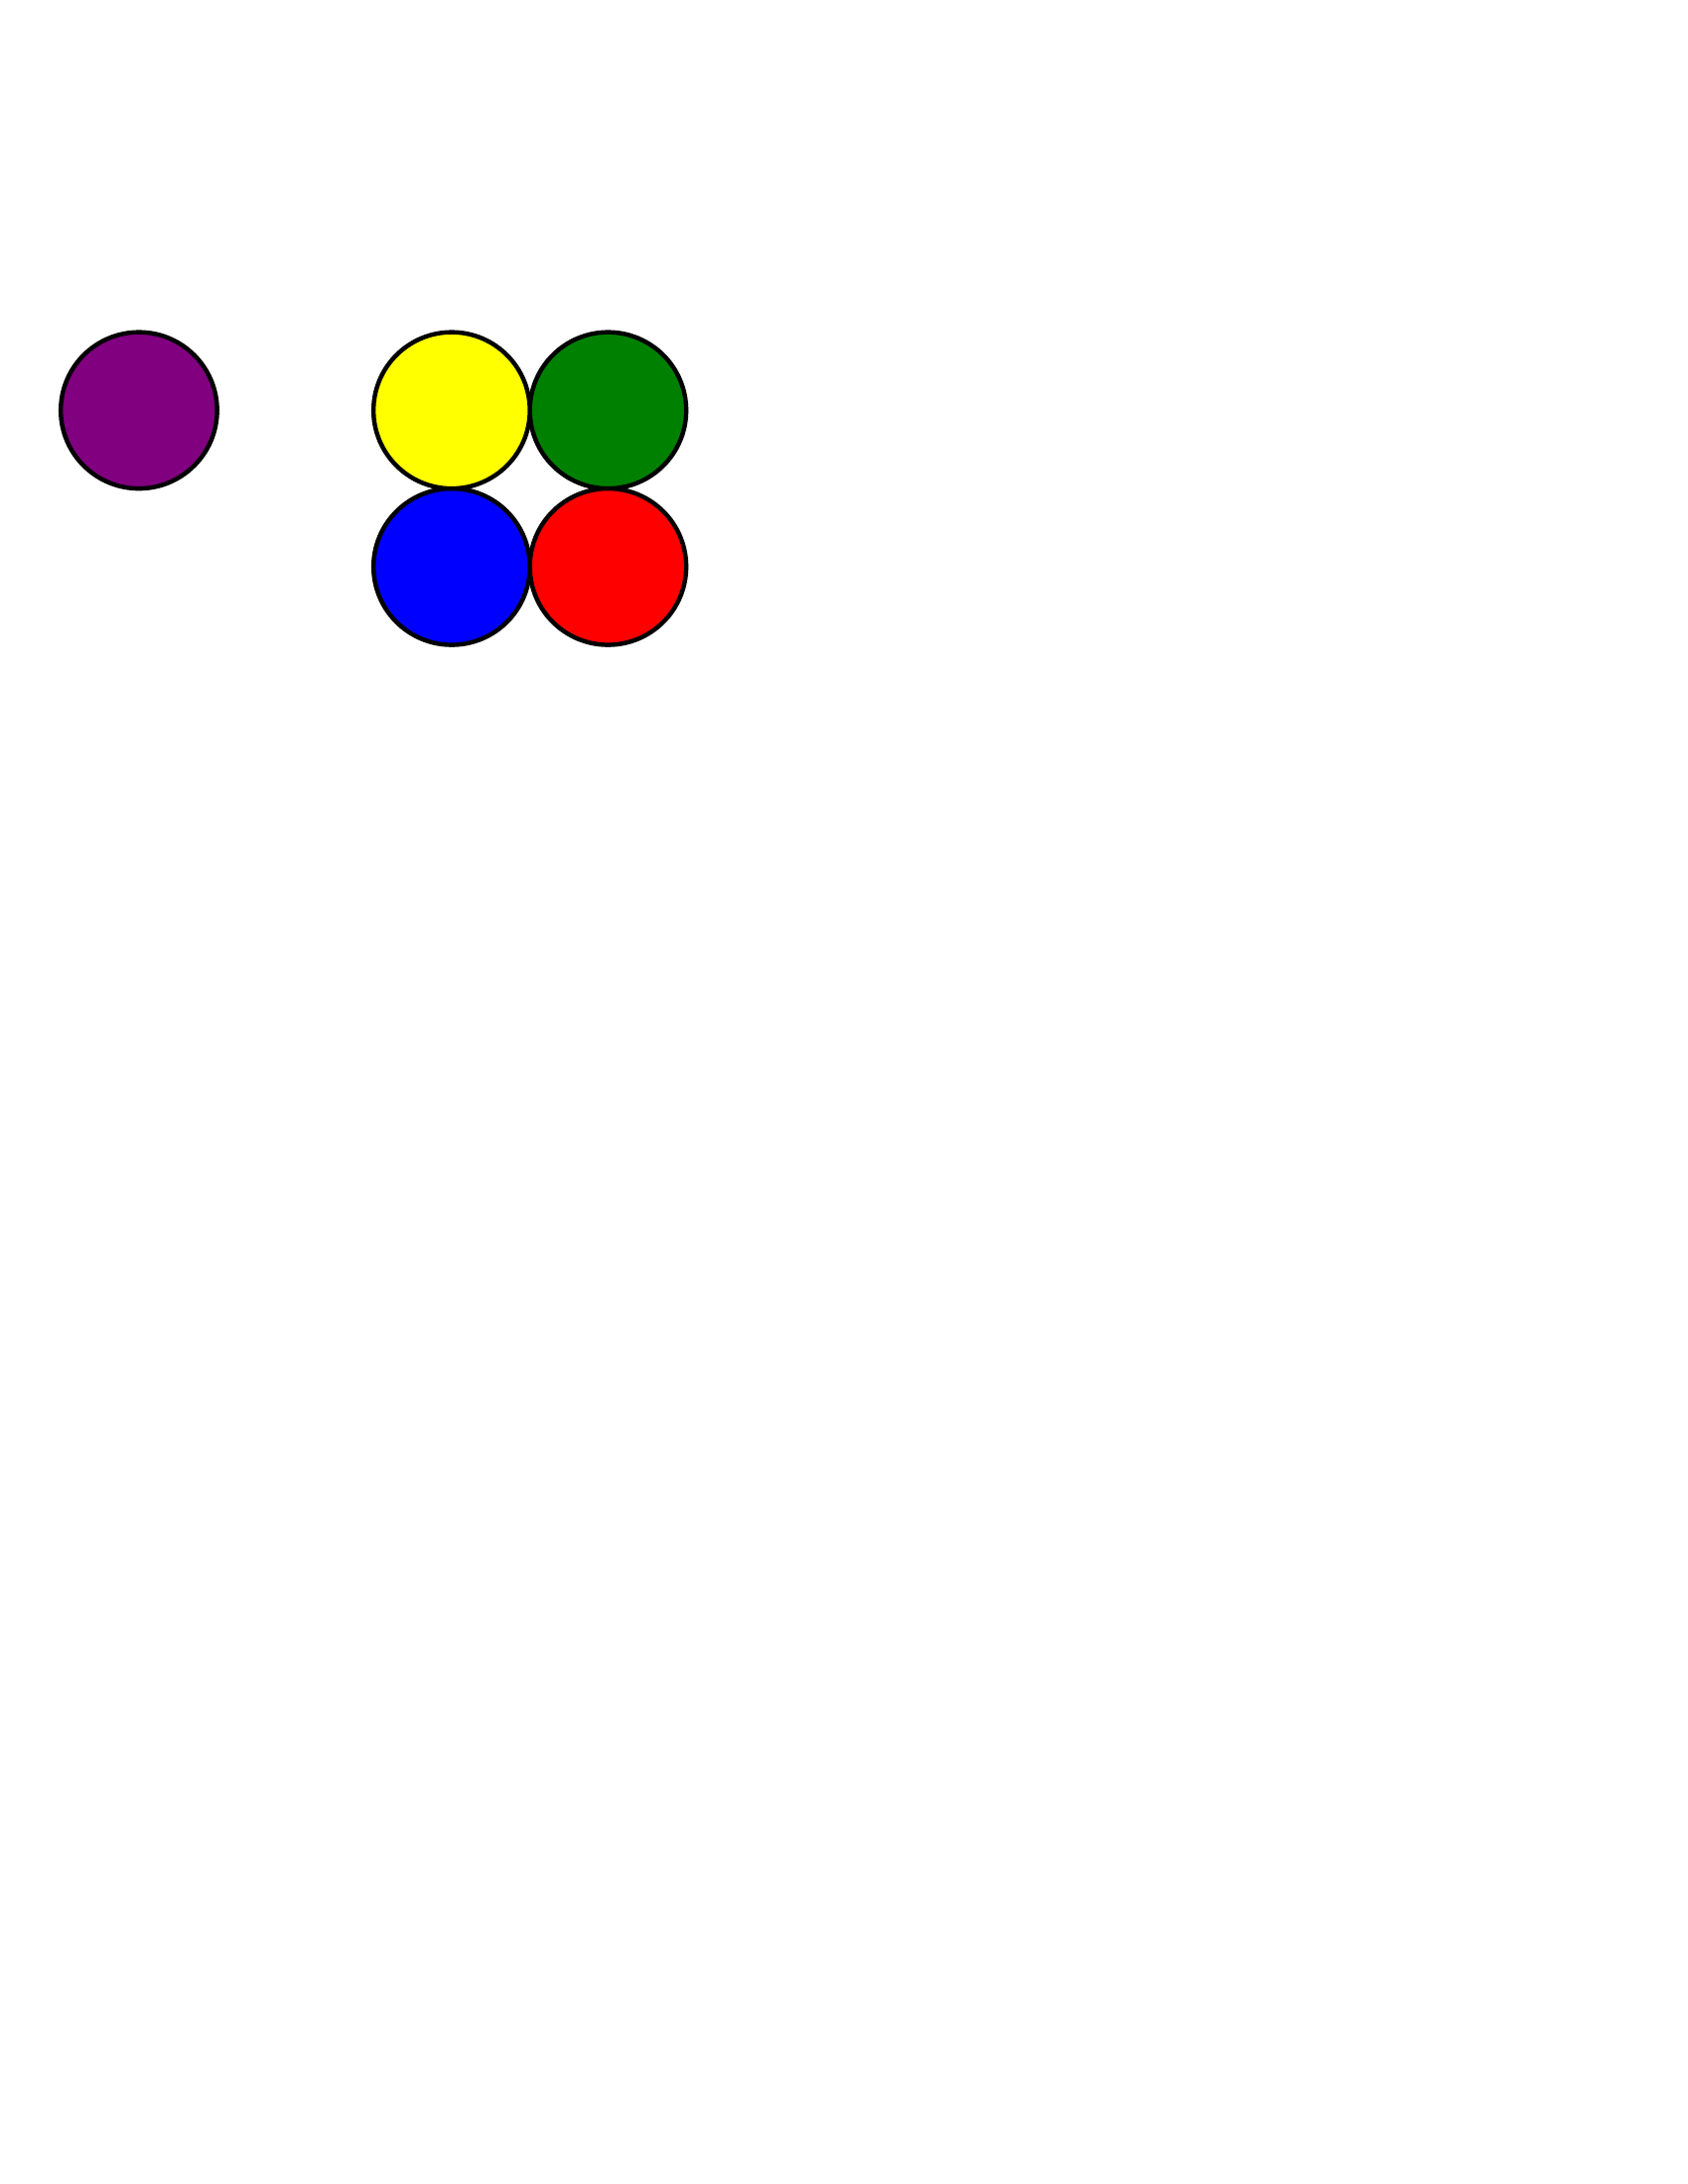
\begin{tikzpicture}[x=1cm, y=1cm]
	\path (-6.25,-6.25) to (6.25,6.25); 

	\node[draw, ultra thick, circle, minimum size=2cm, inner sep=0pt, fill=Blue] at (-1,-1) {};
	\node[draw, ultra thick, circle, minimum size=2cm, inner sep=0pt, fill=Green] at (1,1) {};
	\node[draw, ultra thick, circle, minimum size=2cm, inner sep=0pt, fill=Purple] at (-5,1) {};
	\node[draw, ultra thick, circle, minimum size=2cm, inner sep=0pt, fill=Red] at (1,-1) {};
	\node[draw, ultra thick, circle, minimum size=2cm, inner sep=0pt, fill=Yellow] at (-1,1) {};

\end{tikzpicture}}

%Fourth push action

\newframe
\multiframe{10}{i=0+9}{%
\begin{tikzpicture}[x=1cm, y=1cm]
	\path (-6.25,-6.25) to (6.25,6.25); 

	\node[draw, ultra thick, circle, minimum size=2cm, inner sep=0pt, fill=Blue] at (-1,-1) {};
	\node[draw, ultra thick, circle, minimum size=2cm, inner sep=0pt, fill=Green] at (1,1) {};
	\node[draw, ultra thick, circle, minimum size=2cm, inner sep=0pt, fill=Purple, rotate around={\i:(4,0)}] at (-5,1) {};
	\node[draw, ultra thick, circle, minimum size=2cm, inner sep=0pt, fill=Red] at (1,-1) {};
	\node[draw, ultra thick, circle, minimum size=2cm, inner sep=0pt, fill=Yellow] at (-1,1) {};

\end{tikzpicture}}
\newframe
\multiframe{10}{r=0+0.2}{%
\begin{tikzpicture}[x=1cm, y=1cm]
	\path (-6.25,-6.25) to (6.25,6.25); 

	\node[draw, ultra thick, circle, minimum size=2cm, inner sep=0pt, fill=Blue] at (-1,-1+\r) {};
	\node[draw, ultra thick, circle, minimum size=2cm, inner sep=0pt, fill=Green] at (1,1) {};
	\node[draw, ultra thick, circle, minimum size=2cm, inner sep=0pt, fill=Purple] at (-1,-3+\r) {};
	\node[draw, ultra thick, circle, minimum size=2cm, inner sep=0pt, fill=Red] at (1,-1) {};
	\node[draw, ultra thick, circle, minimum size=2cm, inner sep=0pt, fill=Yellow] at (-1,1+\r) {};

\end{tikzpicture}}
\newframe
\multiframe{10}{r=0+0.1}{%
\begin{tikzpicture}[x=1cm, y=1cm]
	\path (-6.25,-6.25) to (6.25,6.25); 

	\node[draw, ultra thick, circle, minimum size=2cm, inner sep=0pt, fill=Blue] at (-1,1) {};
	\node[draw, ultra thick, circle, minimum size=2cm, inner sep=0pt, fill=Green] at (1,1) {};
	\node[draw, ultra thick, circle, minimum size=2cm, inner sep=0pt, fill=Purple] at (-1,-1) {};
	\node[draw, ultra thick, circle, minimum size=2cm, inner sep=0pt, fill=Red] at (1,-1) {};
	\node[draw, ultra thick, circle, minimum size=2cm, inner sep=0pt, fill=Yellow] at (-1+2*\r,3+2*\r) {};

\end{tikzpicture}}
\newframe
\multiframe{30}{i=0+9}{%
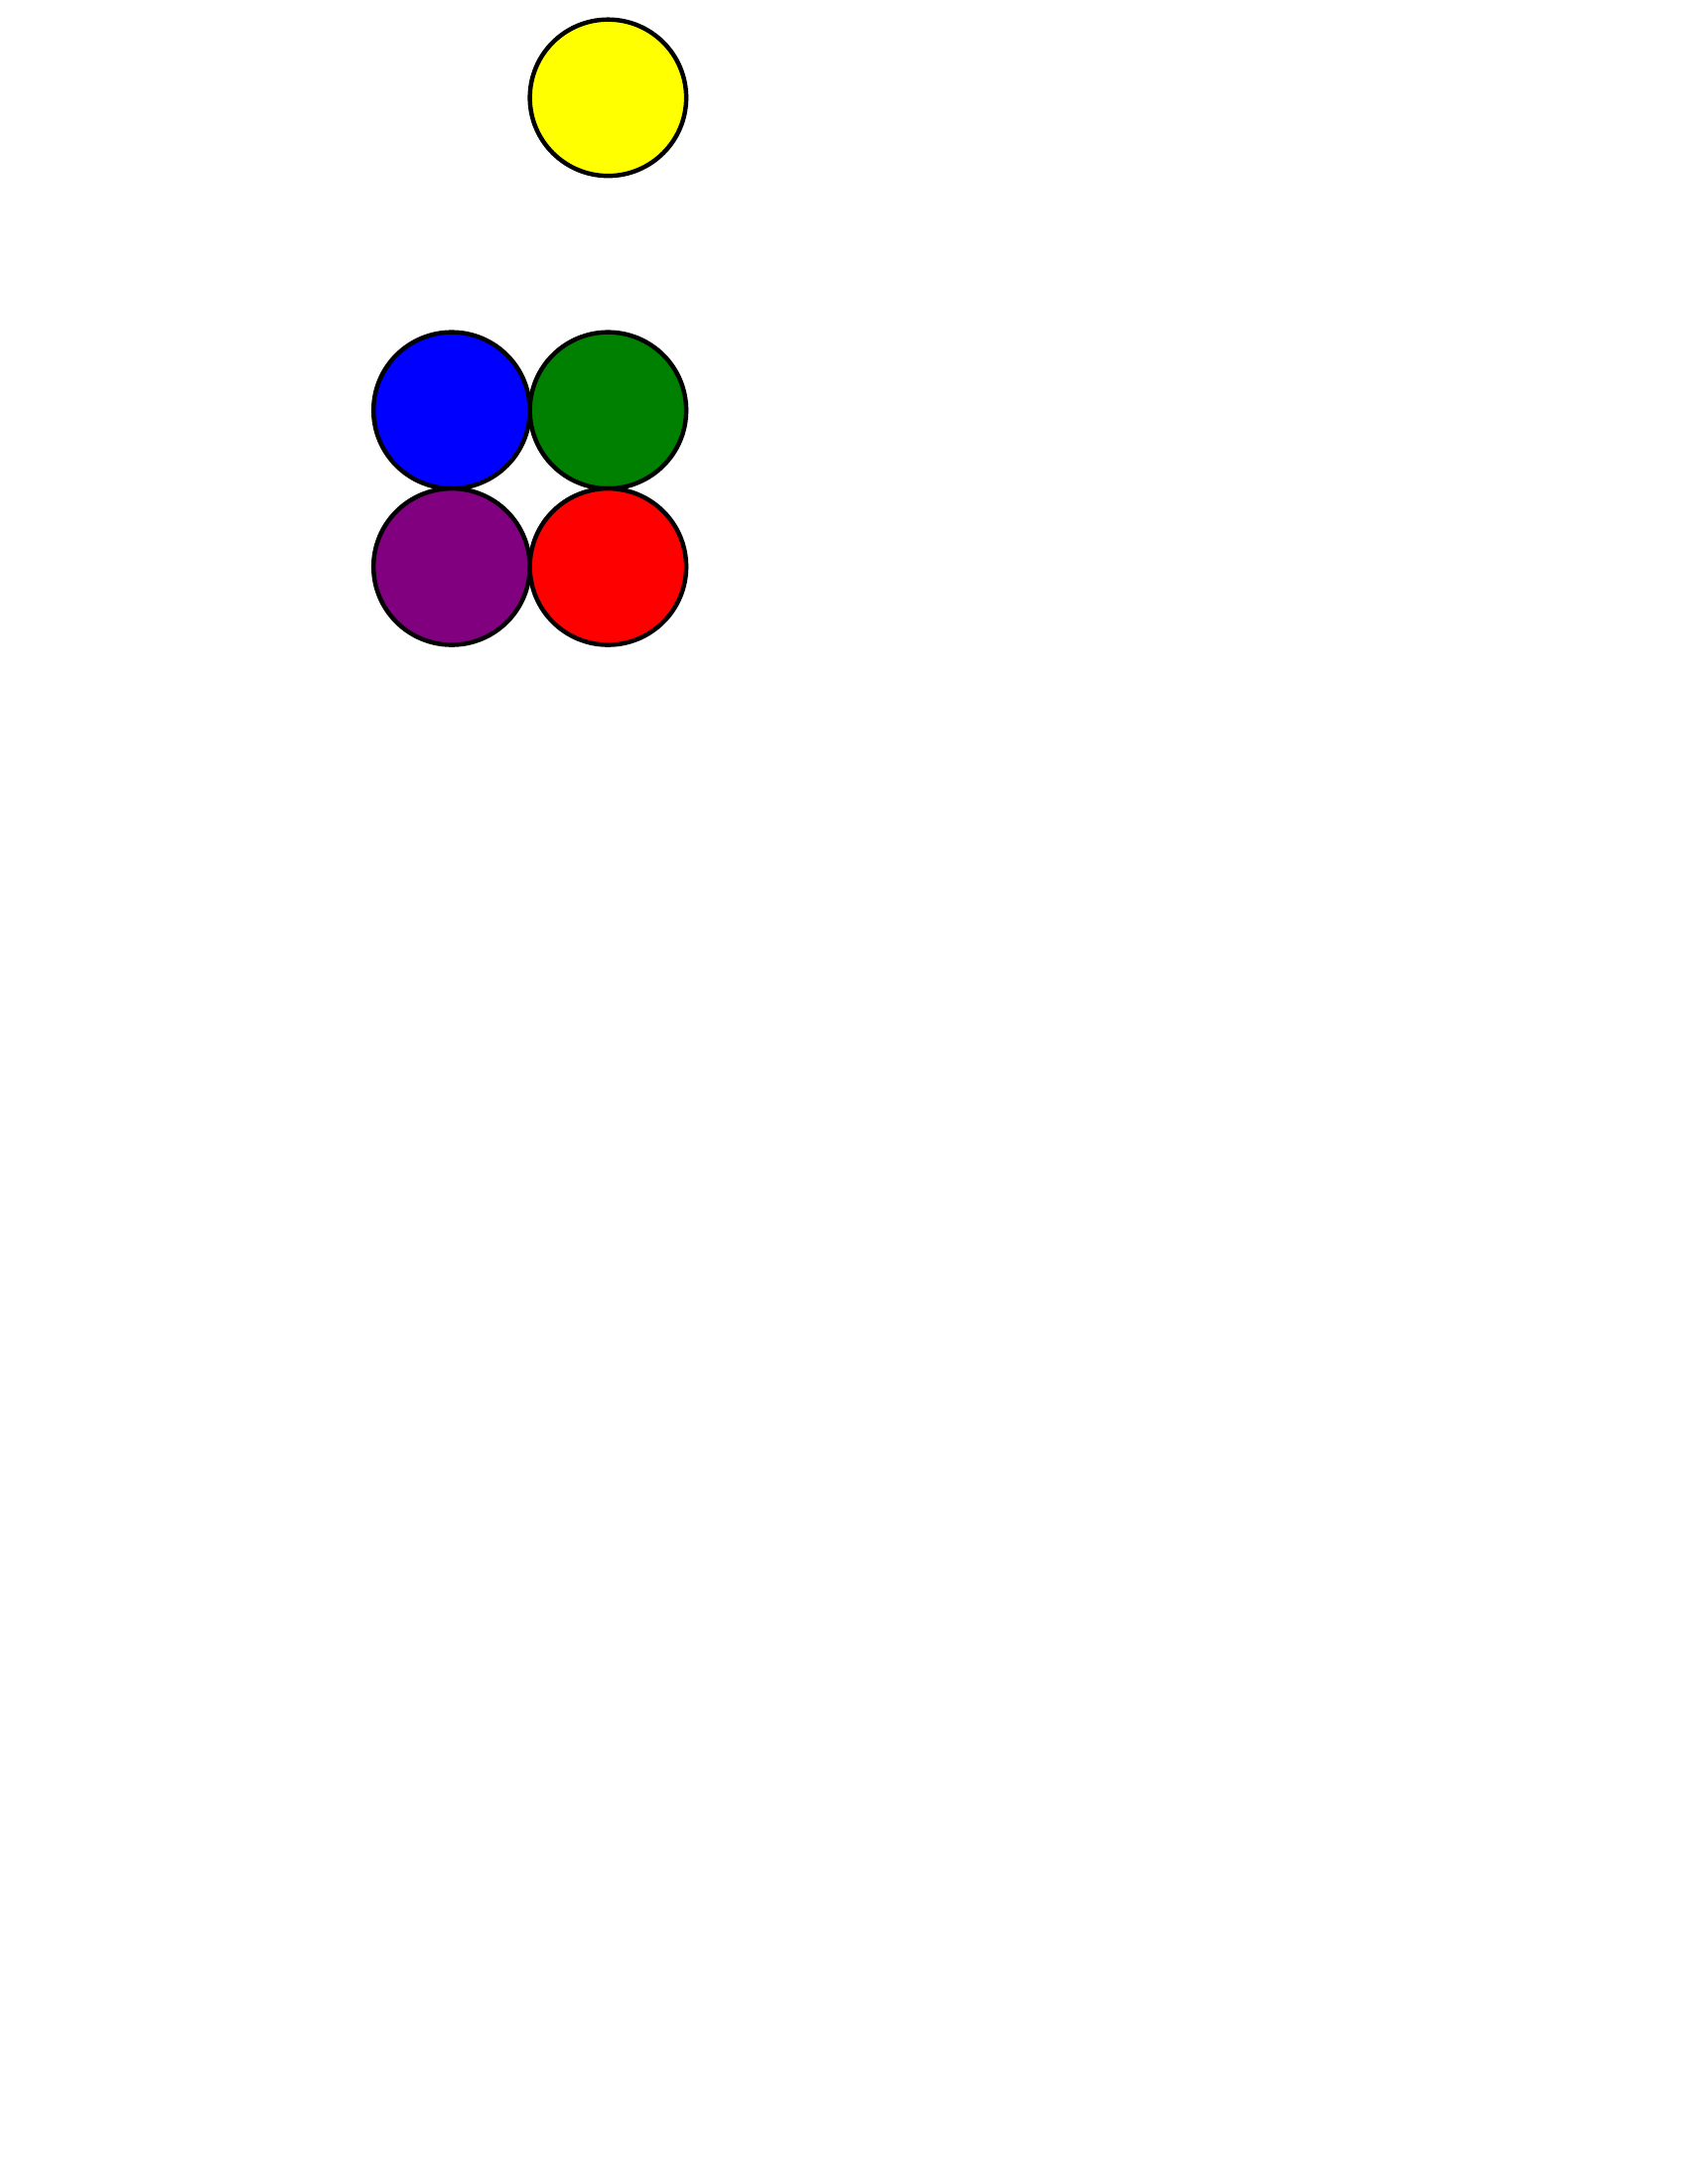
\begin{tikzpicture}[x=1cm, y=1cm]
	\path (-6.25,-6.25) to (6.25,6.25); 

	\node[draw, ultra thick, circle, minimum size=2cm, inner sep=0pt, fill=Blue] at (-1,1) {};
	\node[draw, ultra thick, circle, minimum size=2cm, inner sep=0pt, fill=Green] at (1,1) {};
	\node[draw, ultra thick, circle, minimum size=2cm, inner sep=0pt, fill=Purple] at (-1,-1) {};
	\node[draw, ultra thick, circle, minimum size=2cm, inner sep=0pt, fill=Red] at (1,-1) {};
	\node[draw, ultra thick, circle, minimum size=2cm, inner sep=0pt, fill=Yellow] at (1,5) {};

\end{tikzpicture}}

\end{animateinline}
\end{document}
